% !TEX root = OptimalOffline.tex

We now proceed to relax the condition that the receiver harvests energy only once. The receiever harvests energy equivalent to the amount required to stay on for time $\TRx_i$ at time instances $r_i$. 
We assume that the receiver has an infinite battery capacity. 
Again, since we are considering the offline case, we assume we have knowledge of the receiver energy arrivals non causally. This can be stated as an optimization problem as follows.\\
\begin{problem}
\begin{align}
&\min_{\{\textbf{p},\textbf{s},N\}}			&& T
\\
&\text{subject to} 				&& B(T)=B_0, 
\label{pb2_constraint_bits}
\\
&     										&& U(t)\le \mathcal{E}(t)  		\;\;\;\;\;\; \forall \; t\;\in\;[0,T], \label{pb2_constraint_energy}
\\
&    										&& \displaystyle \sum_{i=1}^k \mathcal{S}_i(s_{i+1} - s_i) + \mathcal{S}_i(t - s_{k+1}) \leq \TRx(t) \\ &&&\forall \; t \; in \; [0,T] \; \text{where} \; k = \max\{i| s_{i+1} \leq t\}.
\label{pb2_constraint_time}
\end{align}
\end{problem}
$\mathcal{S}_i:\mathbb{Z}\rightarrow\{0,1\}$ is a function that takes value $1$ if $p_i>0$ and $0$ otherwise.\\
Our approach to solve this problem will be to use the previously derived algorithm and try to apply it iteratively. Let $O_i$ be the first time instance such that if the receiver is started for the first time at $O_i$ and kept on continuously, then it will be able to stay on for $\TRx(r_i)$ time. It can be easily shown, (and seen in figure \ref{figure_origin_points}) that the receiver will exhaust all its energy at at least one energy arrival epoch $r_m$ when it transmits from $O_i$ for $\TRx(r_i)$ time. For example, in the figure, when the receiver transmits starting from $O_1$, it exhausts all it's energy at $r_1^-$. Since the reciever uses a constant amount of power, $O_i = r_m - \TRx(r_{m-1})$. This can be visualised in figure \ref{figure_origin_points}. Now, we prove the following lemmas.\\

\begin{figure}
\centering
  \centerline{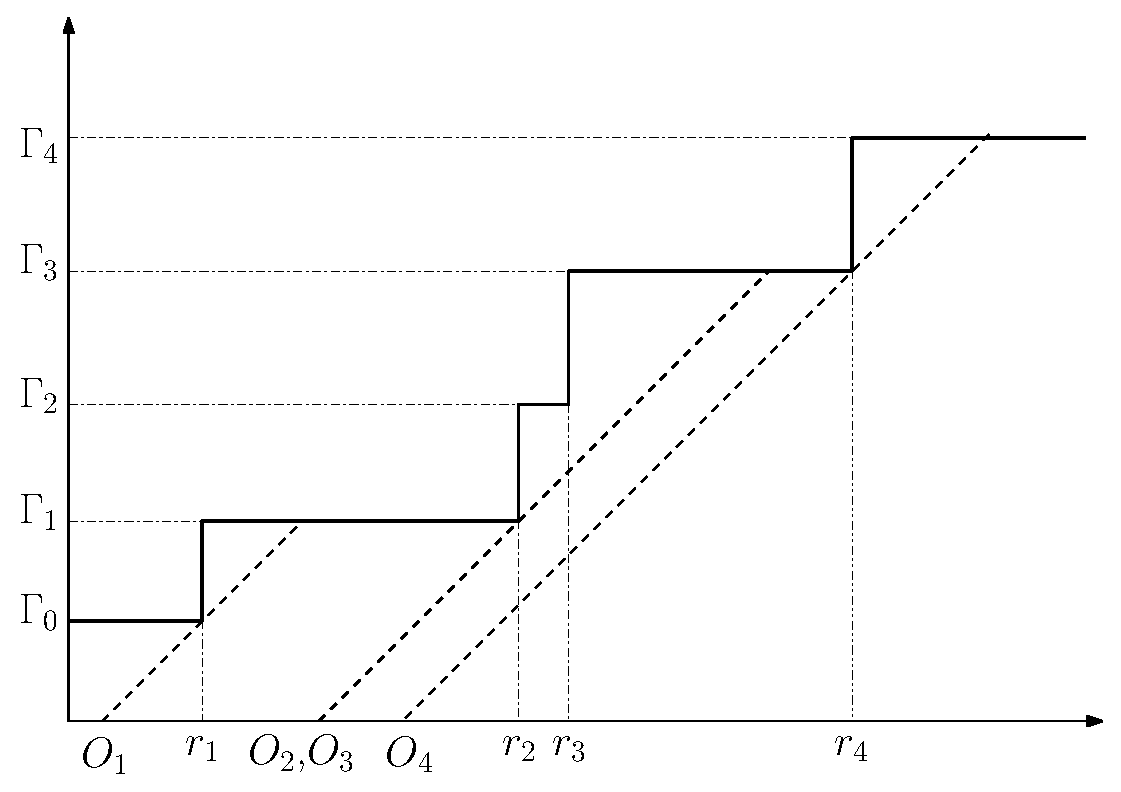
\includegraphics[width=8cm]{origin_points.eps}}
\caption{Figure showing $O_i$'s which represent the first time instances at which the reciever can be kept on continuously for $\TRx(r_i)$ time. Note that $O_2$ and $O_3$ coincide in this example.}\label{figure_origin_points}
\end{figure}

\begin{lemma}
If a policy $\{\bm{p},\bm{s},N\}$ for Problem 2 is optimal, either $s_1 = O_i$ for some $i$, and/or the receiver remains on for exactly $\TRx(r_i)$ time for some $i$.
\label{lemma_origins}
\end{lemma}
\begin{proof}
We shall prove this by contradiction. Suppose a policy $X$ given by $\{\bm{p},\bm{s},N\}$, is optimal and does not satisfy the conditions given in the lemma statement. Then $\TRx(r_{i})<s_{N+1}-s_1<\TRx(r_{i+1})$ for some $i$. Thus, $s_1>O_i$, by definition of $O_i$. Which means that when this policy ends, there will be unspent receiver time remaining. Applying similar arguments as in Lemma \ref{lemma_increase_time} and Lemma \ref{transmission_duration}, we can create a new policy that satisfies all the feasibility constraints and ends before policy $X$.
\end{proof}

Lemma \ref{lemma_origins} gives us an idea about how we can proceed to solve Problem 2. If we shift the origin on both the transmitter and reciever energy arrival energy profiles to time $O_i$, assuming of course that all the transmitter energy and receiver `time' that has arrived before $O_i$ is available starting from $O_i$, and solve this problem using Algorithm 1 (Assuming $\TRx(r_i)$ time is available at the receiver with no additional `time' arrivals), we shall get a policy that either begins transmission at $O_i$ or uses exactly $\TRx(r_i)$ time. This policy abides by the conditions stsated in Lemma \ref{lemma_origins}. We shall refer to this technique as passing an origin $O_i$ and a time $\TRx(r_i)$ into Algorithm 1. Also, the end time of this policy gives us an upper bound to when the optimal policy begins (or ends). We can thus, iterate, over all points $O_i$ in this manner and keep updating our upper bound until we cross the upper bound, and return the most optimal policy that we have attained so far. We now have a preliminary algorithm that terminates in finite time and gives us the optimal policy for Problem 2. We shall prove the optimality of the policy returned in theorem \textbf{?}. First, we make a few more observations about the policies returned by this method. 

\begin{lemma}
A solution $\{\bm{p},\bm{s},N\}$, arrived at by passing $O_i$ and $\TRx(r_i)$ into Algorithm 1 is optimal only if $O_i\leq s_1\leq O_{i+1}$.
\label{lemma_startpoint}
\end{lemma}
\begin{proof}
First we prove that a policy attained by passing $O_i$ and $\TRx(r_i)$ into Algorithm 1 can be optimal only if $O_i\leq s_1\leq O_{i+1}$. Consider a case where $O_i \neq O_{i+1}$ (The result is trivially true for the case where $O_i = O_{i+1}$). Suppose a policy $X$, returned by Algorithm 1 and given by $\{\bm{p},\bm{s},N\}$, is optimal and $s_1 \ge O_{i+1}$. Let $Y$, given by $\{\bm{p'},\bm{s'},N'\}$ be the policy returned when $O_{i+1}$ and $\TRx(r_{i+1})$ are passed into Algorithm 1. Firstly, we note that $X$ is a feasible solution to the optimization problem solved by Algorithm 1 where $O_{i+1}$ and $\TRx(r_{i+1})$ are passed. Therefore, $Y$ must be the same as, or `better' than $X$. Now since $s_1 \neq O_{i+1}$ and $s_{N+1} - s_{N} = \TRx(r_i)$, $X$ cannot be the policy returned by Algorithm 1 when $O_{i+1}$ and $\TRx(r_{i+1})$ are passed (Since such a policy would have to take $\TRx(r_{i+1})$ time). Therefore, policy $Y$ ends strictly before $X$, which proves our result. 
\end{proof}
\begin{lemma}
\label{lemma_first_solution}
Let $X_i$ be the solution returned by Algorithm 1 on passing $O_i$ and $\TRx(r_i)$. The first $X_i$ which begins transmission before $O_{i+1}$ is the optimal solution for Problem 2.
\end{lemma}
\begin{proof}
Let the first $X_i$ having the property stated in the lemma be given by $\{\bm{p},\bm{s},N\}$. Suppose it is not the optimal solution to Problem 2. Let the optimal solution be $Y$, given by  $\{\bm{p'},\bm{s'},N'\}$ . We can divide the proof into two cases. The first where $Y$ begins transmission before $O_i$ and the second where it begins transmission after $O_i$.\\ In the first case, suppose $O_{k}\le s'_1 < O_{k+1}$. Then $\TRx(r_{l})\le s'_{N+1} - s'_1 <\TRx(r_{l+1})$ for some $l<k$. Therefore, $Y$ is a feasible policy for the optimization problem solved by Algorithm 1 when $O_l$ and $\TRx(r_l)$ are passed. On account of the optimality of $Y$ and Algorithm 1, $Y$ will be the solution returned by Algorithm 1. But since $s'_1 > O_{l+1}$ by the condition in the lemma, Lemma \ref{lemma_startpoint} implies that $Y$ cannot be optimal.\\
Now consider the case where $s'_1\ge O_i$. Optimality of $Y$ implies $s'_N+1<s_N+1$. If $s'_1\ge s_1$, then $s'_N+1-s_1\le \TRx(r_i)$, implying (using similar arguments as above) that Algorithm 1 would return $Y$ and not $X$, which is a contradiction. Now if $O_i\le s'_1<s_1$, then $s'_N+1-s_1\le \TRx(r_i)$, since $s_1\le O_{i+1}$ and $\TRx(r_i)$ is the maximum receiver time available. Again, Optimality of $Y$ would contradict the optimality of Algorithm 1.
\end{proof} 

From Lemma \ref{lemma_first_solution}, we have a better method to know when to stop executing our algorithm. We now need only to iterate through the points $O_i$, passing them into Algorithm 1, until we get a policy that starts before $O_{i+1}$. We are assured by Lemma \ref{lemma_startpoint} that such a policy will be optimal.
\begin{table}
\begin{minipage}[b]{8cm}
\caption {Offline algorithm for energy arrival in receiver after time t=0}
\begin{tabular}{p{7cm}}
\hline \textbf{Input}: Bits to transmit $B_0$; $\ETx_i$, $\TRx_i$ for all $i$
\\
\hline
\\
\textbf{Initialize:}
\\ 
$u=\min u_i$ s.t. $\TRx(u_i)g\left( \dfrac{\ETx(u_i)}{\TRx(u_i)} \right) \ge B_0$. $O_f=\infty$.\\ $u_1=min(r_1,t_1),u_2=min(..)$
\\
For all $i$, define $O_i=\min$ $t$ s.t. receiver can be \textit{on} from $t$ to $(t+\TRx(r_i))$, i.e. $x-t \le \TRx(x)$,  $t \le x\le (t+\TRx(r_i))$.
\\
\\
\textbf{if} $u=r_j$ for some $j$  \textbf{then}
\\
\hspace{4mm}$O_l=O_{j}$, $T=\TRx(r_j)$
\\
\textbf{else}
\\
\hspace{4mm}Let $u=t_j$ for some $j$
\\
\hspace{4mm}$u_{j'}=\min r_i$ s.t. $\TRx(r_i)g\Bigg{(} \dfrac{\ETx(t_j)}{\TRx(r_i)}\Bigg{)}\ge B_0$
\\
\hspace{4mm}$O_l=O_{j'}$, $T=\TRx(r_{j'})$.
\\
\textbf{end if}
\\
\textbf{do}
\\
\hspace{4mm}Apply $Algo1(O_l,T)\rightarrow T_{opt}$
\\
\hspace{4mm}$r_k=\max_i r_i $ s.t. $r_i<T_{opt}$ 
\\
\hspace{4mm}\textbf{if} $O_{f} > O_{k}$
\\
\hspace{7mm}$O_{f} = O_{k}$
\\
\hspace{4mm}\textbf{end if}
\\
\hspace{4mm}\textbf{if} hit origin \textbf{then} $l=l-1$ \textbf{else} $l=l+1$
\\
\textbf{while} $O_l \le O_{f}$
\\
\hline
\label{online}
\end{tabular}
\end{minipage}
\end{table}
